\documentclass{standalone}
\usepackage{tikz}
\usepackage{ctex,siunitx}
\setCJKmainfont{Noto Serif CJK SC}
\usepackage{tkz-euclide}
\usepackage{amsmath}
\usetikzlibrary{patterns, calc,3d}
\usetikzlibrary {decorations.pathmorphing,decorations.pathreplacing,decorations.shapes}
\tikzset{label style/.append style={font=\small}}
\begin{document}
\small
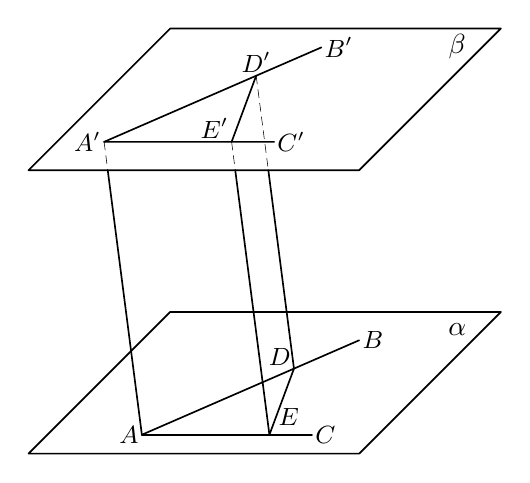
\begin{tikzpicture}[>=latex,scale=1.2,inner sep=1pt]
  \tkzDefPoints{0/0/M,3.5/0/N,5/1.5/P,1.5/1.5/Q,0/3/M'}
  \tkzDefPointsBy[translation=from M to M'](N,P,Q){N',P',Q'}
  \tkzDefPoints{1.2/0.2/A,3.0/0.2/C,3.5/1.2/B,0.8/3.3/A'}
  \tkzDefPointOnLine[pos=0.7](A,B)\tkzGetPoint{D}
  \tkzDefPointOnLine[pos=0.75](A,C)\tkzGetPoint{E}
  \tkzDefPointsBy[translation=from A to A'](B,C,D,E){B',C',D',E'}
  \tkzInterLL(A,A')(M',N')\tkzGetPoint{A''}
  \tkzInterLL(D,D')(M',N')\tkzGetPoint{D''}
  \tkzInterLL(E,E')(M',N')\tkzGetPoint{E''}
  \tkzDrawPolygon[semithick](M,N,P,Q)
  \tkzDrawPolygon[semithick](M',N',P',Q')
  \tkzDrawSegments[semithick](B,A A,C B',A' A',C' D,E D',E' A,A'' D,D'' E,E'')
  \tkzDrawSegments[densely dashed](A',A'' D',D'' E',E'')
  \tkzLabelPoints[right](B,B',C,C')
  \tkzLabelPoints[left](A,A')
  \tkzLabelPoints[above](D')
  \tkzLabelPoints[above right=3pt](E)
  \tkzLabelPoints[above left](D,E')
  \tkzLabelAngle[pos=0.5](Q,P,N){$\alpha$}
  \tkzLabelAngle[pos=0.5](Q',P',N'){$\beta$}
\end{tikzpicture}
\end{document}